
\فصل{روش‌شناسی}
\label{method}
\begin{itemize}
\item
روش
\item
داده‌های مورد نیاز
\item
روش‌های آنالیز
\item
نحوه‌ی تفسیر نتایج
\end{itemize}

\قسمت{ارجاع به مقالات}
نمونه ارجاع به مقاله  \Latincite{Herbert1998}.

\قسمت{جدول}
جدول \ref{t1} نمونه یک جدول است.

\begin{center}
\begin{table}
\centering
\caption {‌جدول نمونه}
%\tabcolsep=0.12cm
\begin{tabular}{cr}
\hline 
متغیّر &  توضیح \\ \hline
$ Y $ &  سرانه‌ی ماحصل اقتصادی \\ 
$ I $ &  درآمد خالص اقتصادی \\ 
$ B $ &  نرخ زاد ولد \\ 
$ D $ &  نرخ مرگ‌ و میر \\ 
$ N $ &  جمعیّت \\ 
$ F $ &  جریان آلاینده‌ها \\ 
$ K $ &  منابع طبیعی \\ 
$ C $ &  هزینه‌ی صرف‌شده برای حفظ محیط‌زیست \\ 
$ P $ &  میزان آلودگی \\  \hline 
\end{tabular}
\label{t1}
\end{table}
\end{center}

\قسمت{تصویر}
شکل \ref{f1} نمونه‌ای از یک تصویر است.

\begin{figure}%[h]
	\centering
	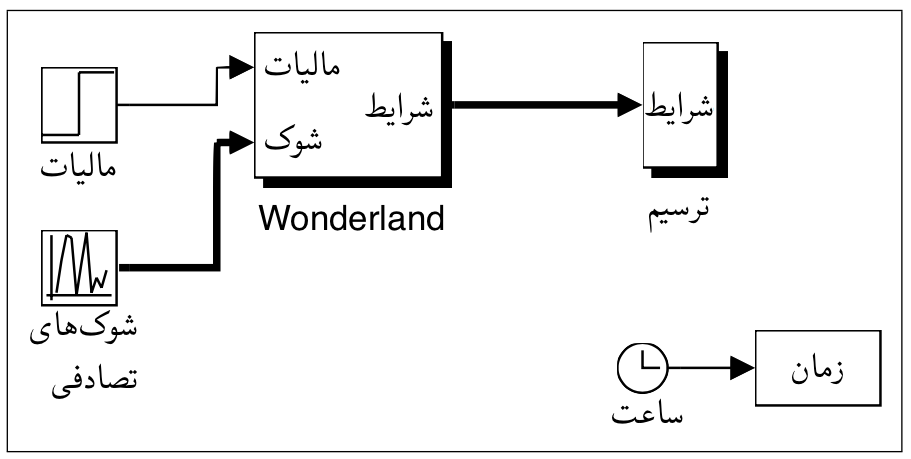
\includegraphics[width=12cm]{Wonderland.png}
	\caption{تصویر نمونه}
	\label{f1}
\end{figure}

\قسمت{معادلات ریاضی}
معادله \ref{e1} نمونه‌ای از یک رابطه ریاضی است.
\begin{equation}
	\label{e1}
	K_{t+1}= \frac{e^{ln(\frac{K_t}{1-K_t}+\delta K_t^\rho - \omega F_t)}}{1+e^{ln(\frac{K_t}{1-K_t}+\delta K_t^\rho - \omega F_t)}}
\end{equation}
 
 